\begin{subsection}{Steps 5 e 6}
    \begin{frame}{DISTILLED-SINGLE-SHOT-DETECTOR (DSSD)}
        \begin{figure}
            \centering
            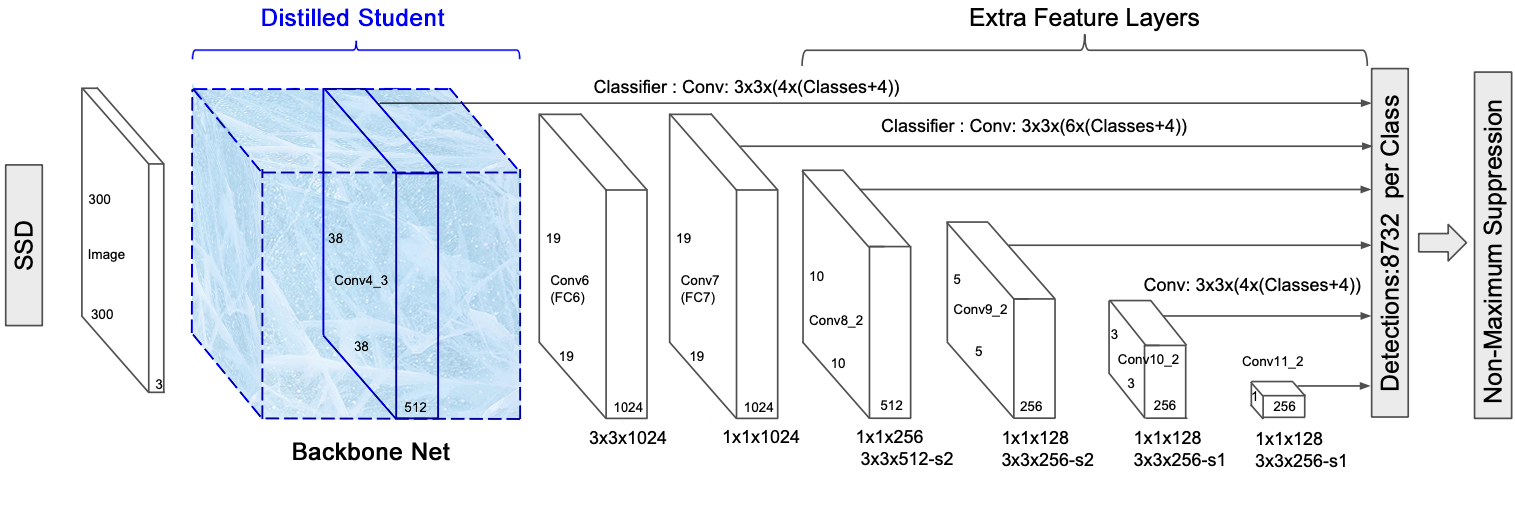
\includegraphics[width = \linewidth]{SSD_architecture_freeze.png}
            \centering
        \end{figure}
        \begin{minipage}{\linewidth}
            \centering
            \begin{minipage}{0.45\linewidth}
                \begin{block}{\centering 5. Integrazione}
                    \centering
                    Studente distillato come rete "{\bfseries{\emph{backbone}}}" nell'architettura {Single-Shot-Detector (SSD)}.    
                \end{block}
            \end{minipage}
            \hspace{0.5cm}
            \begin{minipage}{0.45\linewidth}
                \begin{block}{\centering 6. Freeze}
                    \centering
                    "{\bfseries{\emph{Congelamento}}}" livelli rete \emph{backbone} durante \emph{l'allenamento} del modello (DSSD).
                \end{block}
            \end{minipage}
        \end{minipage}   
    \end{frame}
\end{subsection}
